% !TeX program = xetex
\documentclass[xcolor={table,usenames,dvipsnames}]{beamer}
\usepackage{eso-pic} 
\usepackage[absolute,overlay]{textpos}
\usepackage{colortbl}
\usepackage{fourier}
\usepackage{booktabs}% http://ctan.org/pkg/booktabs
\newcommand{\tabitem}{~~\llap{\textbullet}~~}
\usepackage{tabularx}
\setbeamertemplate{blocks}[rounded][shadow=true]
\let\olditem\item
\renewcommand{\item}{%
\olditem\vspace{0pt}}     
\usepackage{ragged2e}
% Reduce spacing between item levels




\makeatletter
\def\@listii{\leftmargin2em
	\topsep2pt
	\parsep2pt
	\itemsep2pt} % applies to second level itemize
\makeatother


%\definecolor{myblockcolor}{rgb}{1,1,1} % Light cyan, or any color you prefer
%\setbeamercolor{block title}{bg=blue!30,fg=black}
%\setbeamercolor{block body}{bg=myblockcolor,fg=black}

% Define custom title bar color
\definecolor{mytitlecolor}{rgb}{0.4,0.6,0.8} % Adjust as desired

% Set block title color
\setbeamercolor{block title}{bg=mytitlecolor, fg=white}
\setbeamercolor{block title alerted}{bg=mytitlecolor, fg=white}


%\usepackage[round]{natbib} % incompatible avec biblatex
\usepackage{hyperref}
\hypersetup{
    colorlinks=true,
    linkcolor=.,
    filecolor=deepblue,      
    urlcolor=deepblue,
    pdftitle={Overleaf Example},
    pdfpagemode=FullScreen,
    citecolor=deepblue
    }
\definecolor{LightCyan}{rgb}{0.88,1,1}   
\usepackage[justification=centering]{caption}
\captionsetup{font=scriptsize}
\captionsetup[figure]{name=Fig.}
\captionsetup[table]{name=Tab.}
\setbeamertemplate{caption}[numbered]
\usepackage[T1]{fontenc}
\usepackage{ctex}
\UseRawInputEncoding
%\usepackage[backend=bibtex, style=authoryear, natbib=true, sorting=nty, backref=true]{biblatex}
\usepackage[style=authoryear, maxbibnames=99, mincitenames=1, maxcitenames=2, backref=true, hyperref=true, dashed=false, firstinits=true, backend=bibtex, bibencoding=utf8, uniquename=false, uniquelist=false, natbib=true]{biblatex}
\renewcommand*{\bibfont}{\footnotesize}
\setbeamerfont{footnote}{size=\tiny}


% Remove quotation marks from titles
\DeclareFieldFormat[article,incollection,inproceedings,conference]{title}{#1} 
\addbibresource{bibliographie.bib}
\usepackage{soul}




%\usepackage[backend=bibtex,
%style=authoryear,
%natbib=true,
%sorting=nty,
%backref=true
%]{biblatex}

\let\oldnocite\nocite
\makeatletter
\renewcommand*{\nocite}[1]{\oldnocite{#1}\Hy@backout{#1}}
\makeatother

\renewcommand*{\bibfont}{\footnotesize}

\DeclareCiteCommand{\cite}
  {\usebibmacro{prenote}}
  {\usebibmacro{citeindex}%
   \printtext[bibhyperref]{\usebibmacro{cite}}}
  {\multicitedelim}
  {\usebibmacro{postnote}}

\DeclareCiteCommand*{\cite}
  {\usebibmacro{prenote}}
  {\usebibmacro{citeindex}%
   \printtext[bibhyperref]{\usebibmacro{citeyear}}}
  {\multicitedelim}
  {\usebibmacro{postnote}}

\DeclareCiteCommand{\parencite}[\mkbibparens]
  {\usebibmacro{prenote}}
  {\usebibmacro{citeindex}%
    \printtext[bibhyperref]{\usebibmacro{cite}}}
  {\multicitedelim}
  {\usebibmacro{postnote}}

\DeclareCiteCommand*{\parencite}[\mkbibparens]
  {\usebibmacro{prenote}}
  {\usebibmacro{citeindex}%
    \printtext[bibhyperref]{\usebibmacro{citeyear}}}
  {\multicitedelim}
  {\usebibmacro{postnote}}

\DeclareCiteCommand{\footcite}[\mkbibfootnote]
  {\usebibmacro{prenote}}
  {\usebibmacro{citeindex}%
  \printtext[bibhyperref]{ \usebibmacro{cite}}}
  {\multicitedelim}
  {\usebibmacro{postnote}}

\DeclareCiteCommand{\footcitetext}[\mkbibfootnotetext]
  {\usebibmacro{prenote}}
  {\usebibmacro{citeindex}%
   \printtext[bibhyperref]{\usebibmacro{cite}}}
  {\multicitedelim}
  {\usebibmacro{postnote}}

%\DeclareCiteCommand{\textcite}
%  {\boolfalse{cbx:parens}}
%  {\usebibmacro{citeindex}%
%   \printtext[bibhyperref]{\usebibmacro{textcite}}}
%  {\ifbool{cbx:parens}
%     {\bibcloseparen\global\boolfalse{cbx:parens}}
%     {}%
%   \multicitedelim}
%  {\usebibmacro{textcite:postnote}}

%        \DeclareCiteCommand{\textcite}
%        {\usebibmacro{cite:init}%
%            \usebibmacro{prenote}}
%        {\usebibmacro{citeindex}%
%            \printtext[bibhyperref]{\usebibmacro{textcite}}}
%        {}
%        {\printtext[bibhyperref]{\usebibmacro{textcite:postnote}}%
%            \usebibmacro{cite:post}}

%\addbibresource{bibliographie.bib}

% Cannot enable in Xelatex
\usepackage{pgfpages}
% \setbeameroption{hide notes} % Only slides
% \setbeameroption{show only notes} % Only notes
% \setbeameroption{show notes on second screen}

% other packages
\usepackage{latexsym,amsmath,multicol,booktabs,calligra}
\usepackage{graphicx,listings,stackengine}
\usepackage[greek,french]{babel}
\usepackage[LGR,T1]{fontenc}
\usepackage{fontspec}

%\usepackage[sfdefault,light,led=.85]{merriweather} %% Option 'black' gives heavier bold face 


\usepackage[sfdefault]{AlegreyaSans} %% Option 'black' gives heavier bold face
%% The 'sfdefault' option to make the base font sans serif
\renewcommand*\oldstylenums[1]{{\AlegreyaSansOsF #1}}



% Define a command for text in Greek. Replace 'Gentium Plus' with a font of your choice if necessary.
%\newfontfamily\greekfont{Gentium Plus}
%\newcommand{\textgreek}[1]{{\greekfont #1}}

\DefineBibliographyStrings{french}{%
  backrefpage = {voir p\adddot},%
  backrefpages = {voir pp\adddot}%
}
\DeclareFieldFormat{pagerefformat}{\mkbibparens{{\color{red}\mkbibemph{#1}}}}
\renewbibmacro*{pageref}{%
  \iflistundef{pageref}
    {}
    {\printtext[pagerefformat]{%
       \ifnumgreater{\value{pageref}}{1}
         {\bibstring{backrefpages}\ppspace}
         {\bibstring{backrefpage}\ppspace}%
       \printlist[pageref][-\value{listtotal}]{pageref}}}}
\usepackage{wasysym}
% Enable only in Xelatex
 \usepackage{pstricks}

\author[Ljudmila PETKOVIC]{\small \textbf{Ljudmila PETKOVIC}\textsuperscript{1,2,3,4}\\\medskip{\footnotesize\texttt{prenom.nom@sorbonne-universite.fr}}}
\title[Extraction de phrases-clés : évaluations quantitative et qualitative]{\fontsize{13pt}{13pt}\selectfont Extraction de phrases-clés à partir du corpus Charcot : évaluations quantitative et qualitative}
%\subtitle{Approche \textit{PatternRank}}
\institute [JE \og{}Humanités numériques\fg{}] {\tiny \textsuperscript{1} Sorbonne Université, Faculté des Lettres, \textsc{UFR} Littératures françaises et comparée, \textsc{ED III} (\textsc{ED019})\\\textsuperscript{2} Sorbonne Université, Centre d'étude de la langue et des littératures françaises (\textsc{CELLF}), \textsc{UMR 8599}\\\textsuperscript{3} Sorbonne Université, Observatoire des textes, des idées et des corpus (\textsc{ObTIC})\\\textsuperscript{4} Sorbonne Université, \textsc{UFR} Sociologie et Informatique pour les Sciences Humaines}
\date[Séminaire doctoral \textsc{ObTIC}, 02/05/2025]{\scriptsize Séminaire doctoral \textsc{ObTIC} \\\textsc{SCAI}, salle du Conseil\\Paris, le 2 mai 2025}
\usepackage{YTU}

% defs
\def\cmd#1{\texttt{\color{red}\footnotesize $\backslash$#1}}
\def\env#1{\texttt{\color{blue}\footnotesize #1}}
\definecolor{deepblue}{rgb}{0,0,0.5}
\definecolor{deepred}{rgb}{0.6,0,0}
\definecolor{deepgreen}{rgb}{0,0.5,0}
\definecolor{halfgray}{gray}{0.55}
\definecolor{warmblack}{rgb}{0.0, 0.26, 0.26}
\newcommand{\bolder}[1]{{\color{purple}\bfseries#1}}
\lstset{
    basicstyle=\ttfamily\small,
    keywordstyle=\bfseries\color{deepblue},
    emphstyle=\ttfamily\color{deepred},    % Custom highlighting style
    stringstyle=\color{deepgreen},
    numbers=left,
    numberstyle=\small\color{halfgray},
    rulesepcolor=\color{red!20!green!20!blue!20},
    frame=shadowbox,
}
% \logo{%
%     
\includegraphics[width=1cm,height=1cm,keepaspectratio]{pic/obtic.jpg}~%
%     
\includegraphics[width=1cm,height=1cm,keepaspectratio]{pic/Lettres_su_logo.png}~%
% }
\usepackage{enumerate}
\setbeamertemplate{section in toc}{\hspace*{1em}\inserttocsectionnumber.~\inserttocsection\par}
\setbeamertemplate{subsection in toc}{\hspace*{2em}\inserttocsectionnumber.\inserttocsubsectionnumber.~\inserttocsubsection\par}
\renewcommand*{\bibfont}{\scriptsize}



\let\oldfootnotesize\footnotesize
\renewcommand*{\footnotesize}{\oldfootnotesize\scriptsize}

%\setbeamertemplate{itemize/enumerate body begin}{\small}
\setbeamertemplate{itemize/enumerate subbody begin}{\small}
%
%\newcommand{\leftquote}{{\fontfamily{lmr}\selectfont\textquotedblleft}}
%\newcommand{\rightquote}{{\fontfamily{lmr}\selectfont\textquotedblright}}
%\newcommand{\leftguillemet}{{\fontfamily{lmr}\selectfont\guillemotleft}}
%\newcommand{\rightguillemet}{{\fontfamily{lmr}\selectfont\guillemotright}}


\setbeamertemplate{itemize subitem}{\textcolor{blue}{$\circ$}}




\begin{document}

\begin{frame}
    \titlepage
\begin{figure}
    \centering
    
    
\includegraphics[width=2cm,height=1cm,keepaspectratio]{pic/Lettres_su_logo.png}~\hspace*{0.5cm}%\includegraphics{}
    
\includegraphics[width=2cm,height=1cm,keepaspectratio]{pic/cellf.png}~\hspace*{0.5cm}%
    
\includegraphics[width=3cm,height=1cm,keepaspectratio]{pic/obtic.jpg}~%

\end{figure}
    
    \begin{note}
        {Introduce your self}
    \end{note}

c\end{frame}

\section*{Table des matières}
\begin{frame}{Table des matières}
	\tableofcontents[subsectionstyle=show/show]
\end{frame}



\section[Contributions de Charcot]{Contributions de Charcot}
\begin{frame}{Termes inventés par Charcot : référence}
	\begin{table}[h]
		\small
			\begin{tabular}{rl}
			nom traditionnel & nom moderne / alternatif \\
			\hline
			\bolder{paralysie agitante} & maladie de Parkinson\\
			\bolder{ataxie locomotrice progressive} & \textit{tabes dorsalis}\\
			\bolder{arthropathies tabétiques} & arthropathie de Charcot\\
			\bolder{trépidation épileptoïde du pied}  & \textit{clonus}\\
			\bolder{sclérose en plaques disséminées} & sclérose multiple\\
			\bolder{sclérose latérale amyotrophique} & maladie de Charcot / Lou Gehrig\\
			\bolder{idée(s) fixe(s)}, \bolder{maladie des tics convulsifs} & syndrome de Tourette\\
			\bolder{chorées}, \bolder{athétose}  &  mouvements involontaires	\\
			\bolder{astasie-abasie} & incapacité d'être debout / de marcher\\
			\bolder{atrophie musculaire progressive} & maladie Charcot-Marie-Tooth
		\end{tabular}
	\end{table}

	\begin{flushright}
		\scriptsize
		 (\citealp{walusinski,camargo2023}) 
	\end{flushright}
	\medskip
	\begin{flushright}
		\footnotesize
			\begin{tabular}{ll}
			$\neq$ termes transmis : & \textcolor{deepblue}{\textbf{hystérie}}\\ & \textcolor{deepblue}{\textbf{épilepsie}} \\ & \textcolor{deepblue}{\textbf{hypnose}}\\
			& \textcolor{deepblue}{\textbf{athétose}}
		\end{tabular}

	\end{flushright}


\end{frame}


%\begin{frame}{Approches comparées}
%	\begin{enumerate}
%		\item \textcolor{deepblue}{\textbf{\texttt{TermSuite}}} \citep{cram2016terminology}
%		\begin{itemize}
%			\item linguistique, à base de règles $\rightarrow$ TD-IDF
%		\end{itemize} 
%		\item \textcolor{deepblue}{\textbf{TF-IDF, BM25}}\footnote{\url{https://github.com/ljpetkovic/Charcot_circulations}} \citep{robertson1976relevance}  
%		\begin{itemize}
%			\item statistique
%		\end{itemize}
%		\item \textcolor{deepblue}{\textbf{\textit{PatternRank}}} \citep{schopf2022}\footnote{\url{https://github.com/ljpetkovic/Seminaire_doctoral_ObTIC_130325/blob/main/0_main.pdf}}
%		\begin{itemize}
%			\item apprentissage profond
%			\item \texttt{keybert} + \texttt{keyphrase-vectorizers}
%			\item utilisation des étiquettes POS
%		\end{itemize} 
%	\end{enumerate}
%	
%	\begin{block}{\vspace*{-0.6mm}}
%			Traitements effectués en local (1,2) et \textit{via} la plateforme MeSU\footnote{\url{https://sacado.sorbonne-universite.fr/fr/plateforme-mesu/}} (3).
%	\end{block}
%
%\end{frame}

\section[Évaluation quantitative]{Évaluation quantitative}
\begin{frame}{Comparaison des approches d'extraction des phrases-clés}
	Critères :
	\begin{itemize}
		\item prise en compte des termes traditionnels ou de leurs synonymes
		\begin{itemize}
			\item référence : grand dictionnaire terminologique -- \textit{La vitrine linguistique}\footnote{\url{https://vitrinelinguistique.oqlf.gouv.qc.ca/}}
				\begin{itemize}
					\item ex. \textit{paralysie agitante} $\rightarrow$ \textit{maladie de Parkinson}
				\end{itemize}
		\end{itemize}
					\item recenser le score le plus élevé sur le terme ou sur son synonyme
					\item méthodes classiques \textit{vs.} celles de l'état de l'art
	\end{itemize}
	
	\textit{NB} : termes \og{}imbriqués\fg{}, contenant eux-mêmes d'autres termes :
	\begin{itemize}
		\item \textit{SEP} : \textit{nystagmus} + \textit{tremblement} + \textit{embarras parole} (bégaiement)
	\end{itemize}
	\end{frame}
	
	
	% Tableau Charcot
	\begin{frame}{Le domaine potentiellement impactant : \textbf{hystérie}}
		\vspace*{-3mm}
		\begin{table}[h]
			\resizebox{\textwidth}{!}{%
				\centering
				\begin{tabular}{|l|r|r|r|r|r|}
					\hline
					\multicolumn{1}{|c|}{\textbf{Terme}}
					&	\multicolumn{1}{c|}{\textbf{TF-IDF} (\textit{TermSuite})} & 	\multicolumn{1}{c|}{\textbf{TF-IDF}} & 	\multicolumn{1}{c|}{\textbf{BM25}} & 	\multicolumn{1}{c|}{\textit{\textbf{PatternRank}}} & \multicolumn{1}{c|}{\textbf{Moyenne}} \\
					\hline
					\textit{maladie de Parkinson} & NA  & 0,2478 & 0,2397  & 0,7926 &  0,3200 \\
					\textit{ataxie locomotrice progressive} & 0,1981  & 0,4114 & 0,2313 &  0,7912 & 0,408 \\
					\textit{arthropathies tabétiques} & 0,4424 & 0,1655 & 0,337 & 0,8050 & 0,4375 \\
					\textit{trépidation épileptoïde du pied} & 0,0379 & 0,2581 & 0,053 & 0,7581 & 0,2768 \\
					\textit{sclérose en plaques disséminées} & NA & 0,2935 & 0,4812 & 0,7611 & 0,3840 \\
					\textit{tremblement} & NA & 0,2712 & 0,0213 &  0,7834 & 0,2690 \\
					\textit{nystagmus} & NA & 0,2142 & 0,0488 & 0,7683 & 0,2578 \\
					\textit{embarras parole} & NA & 0,0724 & 0,9143 & 0,8159 & 0,4507 \\
					\textit{sclérose latérale amyotrophique} & NA & 0,3287 & 0,1152 & 0,7514 & 0,2988 \\
					\textit{tics convulsifs} & 0,0670 & 0,2273 & 0,1696 & 0,8073 & 0,3178\\
					\textit{atrophie musculaire progressive} & 0,1161 & 0,2321 & 0,0797 & 0,7874 & 0,3038 \\
					%		\textit{abasie} & NA & NA & 0,0445 & 0,3325\\
					\textit{aphasie} & 0,1722 & 0,345 & 0,0289 & 0,7824 & 0,3321 \\
					\textit{astasie-abasie} & 0,1281 & 0,7022 & 0,1912 & 0,7891 & 0,4527 \\
					\textit{athétose} & NA & 0,226 & 0,0797 & 0,7910 & 0,2742\\
					\textit{chorées} & 0,1593 & 0,1933 & 0,0213 & 0,8030 & 0,2942 \\
					\rowcolor{yellow!30}\textit{hystérie} & 0,6892 & 0,5407 & 0,0213 & 0,8194 & \bolder{0,5177} \\
					\textit{épilepsie} & 0,0062 & 0,534 & 0,0213 & 0,8170 & 0,3446 \\
					\textit{hypnose} & 0,0311 & 0,4294 & 0,0994 & 0,7955 & 0,3389\\
					\textit{systématisation de l'organisation de la moëlle épinière} & NA & 0 & 0 & NA & 0 \\
					\textit{localisations cérébrales} & NA & 0,27 & 0,0943 & 0,7493 & 0,2784 \\
					\hline
				\end{tabular}
			}
			\caption{Les scores de pertinence pour les termes de référence à partir du corpus \og{}Charcot\fg{}.}
		\end{table}
		{\small Moyenne pour tous les termes combinés : 0,3280}
	\end{frame}
	
	
	% Tableau Autres
	
	\begin{frame}{Autre domaine potentiellement impactant : \textbf{syndrome de Tourette}}
	 
	
	\begin{table}[h]
		  \resizebox{\textwidth}{!}{%
		\centering
		\begin{tabular}{|l|r|r|r|r|r|}
		\hline
		\multicolumn{1}{|c|}{\textbf{Terme}}
		 &	\multicolumn{1}{c|}{\textbf{TF-IDF} (\textit{TermSuite})} & 	\multicolumn{1}{c|}{\textbf{TF-IDF}} & 	\multicolumn{1}{c|}{\textbf{BM25}} & 	\multicolumn{1}{c|}{\textit{\textbf{PatternRank}}} & \multicolumn{1}{c|}{\textbf{Moyenne}} \\
		\hline
		\textit{maladie de Parkinson} & 0,05 & 0,0775 & 0,333 & 0,7936 & 0,3135  \\
		\textit{ataxie locomotrice progressive} & 0,32 & 0,0386 & 0,4877 &  0,7431 & 0,3974 \\
		\textit{arthropathies tabétiques} & 0,33 & 0,0934 & 0,4928 & 0,7506 & 0,4167 \\
		\textit{trépidation épileptoïde du pied} & 0,0198 & 0,1227 & 0,2919 & 0,7597 & 0,2985 \\
		\textit{sclérose en plaques disséminées} & NA  & 0,178 & 0,8089 & NA & 0,2467 \\
		\textit{tremblement} & NA & 0,1686 & 0,0362 & 0,7683 & 0,2432 \\
		\textit{nystagmus} & 0,0243 & 0,1326 & 0,146 & 0,7474 & 0,2626 \\
		\textit{embarras parole} & NA & NA & 0,0018 & NA & 0,2341 \\
		\textit{sclérose latérale amyotrophique} & NA & 0,044 & 0,6586 & NA & 0,1757 \\
		\rowcolor{yellow!30}\textit{tics convulsifs} & NA & 0,1293 & 0,8385 & 0,8331 & \bolder{0,4502}\footnote{Le score le plus élevé parmi les termes \textbf{inventés} par Charcot $\neq$ \textit{hypnose}.} \\
		\textit{atrophie musculaire progressive} & 0,40 & 0,1118 & 0.3489 & 0,8053 & 0,4165 \\
%		\textit{abasie} & NA & NA & 0,0445 & 0,3325\\
		\textit{aphasie} & 0,0587 & 0,2245 & 0,1334 & 0,7960 & 0,3031 \\
		\textit{astasie-abasie} & NA & 0,0478 & 0,3565 & 0,7375 & 0,2855 \\
		\textit{athétose} & NA & 0,2029 & 0,274 & 0,8068 & 0,3209 \\
		\textit{chorées} & NA & 0,1336 & 0,0701 & 0,8047 & 0,2521 \\
		\textit{hystérie} & 0,2724 & 0,3711 & 0,0442 & 0,8018 & 0,3723 \\
		\textit{épilepsie} & NA & 0,164 & 0,0247 & 0,8199 & 0,2521 \\
		\textit{hypnose} & 0,3543 & 1 & 0,2922 & 0,7738 & 0,6050 \\
		\textit{systématisation de l'organisation de la moëlle épinière} & NA & NA & NA & 0,7550 & 0,1888 \\
		\textit{localisations cérébrales} & 0,43 & 0,034 & 0,3017 & 0,8090 & 0,3937 \\
		\hline
		\end{tabular}
	}
		\caption{Les scores de pertinence pour les termes de référence à partir du corpus \og{}Autres\fg{}.}
	\end{table}
	{\small Moyenne pour tous les termes combinés : 0,3214}
\end{frame}





\section[Évaluation qualitative]{Évaluation qualitative}

\begin{frame}{Analyse des concordances des termes médicaux}
	Analyses effectuées dans \textsc{TXM}.
	\begin{itemize}
		\item on utilise un terme dans le contexte où on cite Charcot
		\begin{itemize}
			\item terme traditionnel (ex. \textit{paralysie agitante})
			\item synonyme ou terme relevant du champ conceptuel en question
			\begin{itemize}
				\item ensembles de mots liés à un certain concept \citep{costachescu2024}\\
				\textit{pied tabétique} $\rightarrow$ forme particulière d'\textit{arthropathies tabétiques}
			\end{itemize}
		\end{itemize}
	\end{itemize}
	\begin{alertblock}{Exemple}
		\texttt{([word = "paralysie"] [word = "agitante"] []* [word = "Charcot"] | [word = "Charcot"] []* [word = "paralysie"] [word = "agitante"]) within p}
				\begin{itemize}
					\item repérer toutes les occurrences dans un paragraphe où \textit{paralysie agitante} et \textit{Charcot} apparaissent dans n'importe quel ordre, séparés par 0 ou plusieurs mots
		\end{itemize}
	\end{alertblock}
\end{frame}
%\begin{frame}{Références à Charcot}
%\bolder{maladie de Parkinson}
%	\bigskip
%	
%	\begin{block}{\vspace*{-0.6mm}}
%		\footnotesize
%		\justifying
%		[$\dots$] \textbf{paralysie agitante} que \textbf{Charcot} a eu raison de dénommer \underline{maladie de Parkinson}, terme qui a le double avantage [$\dots$] de rendre hommage au médecin anglais, qui en a, pour la première fois, donné, en 1817, une description	précise, quoique incomplète, sur certains points.
%	\end{block}
%	
%	\begin{block}{\vspace*{-0.6mm}}
%		\footnotesize
%		\justifying
%		\textbf{Charcot}, d'ailleurs, ne considérait pas la \underline{maladie de Parkinson} comme fatalement incurable.
%	\end{block}
%	
%	\begin{block}{\vspace*{-0.6mm}}
%		\footnotesize
%		\justifying
%		Il est des cas où ce \underline{tremblement parkinsonien} était provoqué par
%		l'hystérie, tels sont les cas de \textbf{Charcot},[$\dots$]
%	\end{block}
%	
%	\begin{block}{\vspace*{-0.6mm}}
%		\footnotesize
%		\justifying
%		[$\dots$] maladie de Parkinson [$\dots$] appartient, elle aussi, au type d'extension. Elle a été présentée par M. \textbf{Charcot} [$\dots$]
%	\end{block} 
%	
%	\begin{block}{\vspace*{-0.6mm}}
%		\footnotesize
%		\justifying
%		[$\dots$] ce contraste dans la \underline{maladie de Parkinson} ; \textbf{Charcot} l'a constaté.
%	\end{block}
%	
%	\begin{block}{\vspace*{-0.6mm}}
%		\footnotesize
%		\justifying
%		\underline{maladie de Parkinson} [$\dots$] comme disait \textbf{Charcot}, en paraphrasant un mot de Parkinson [$\dots$]
%	\end{block}
%\end{frame}
%
%\begin{frame}{Références à Charcot}
%	\bolder{ataxie locomotrice progressive}
%	\begin{block}{\vspace*{-0.6mm}}
%		\footnotesize
%		\justifying
%		[$\dots$] \underline{ataxie locomotrice progressive}, constatée par douze médecins, parmi lesquels, [$\dots$] MM. \textbf{Charcot}
%	\end{block}
%	
%		\begin{block}{\vspace*{-0.6mm}}
%		\footnotesize
%		\justifying
%		[$\dots$] C'est dans la substance grise, dit M. \textbf{Charcot}, [$\dots$] le point de départ de [$\dots$] l'\underline{ataxie}
%	\end{block}
%	
%			\begin{block}{\vspace*{-0.6mm}}
%		\footnotesize
%		\justifying
%		[$\dots$] \textbf{Charcot} a observée sur le trajet de l'un des nerfs sciatiques chez une femme atteinte d'\underline{ataxie locomotrice}
%	\end{block}
%	
%				\begin{block}{\vspace*{-0.6mm}}
%		\footnotesize
%		\justifying
%		[$\dots$] arthropathies [$\dots$] de l'\underline{ataxie locomotrice}, [$\dots$] signalées, pour la première fois, par M. \textbf{Charcot}.
%	\end{block}
%	
%					\begin{block}{\vspace*{-0.6mm}}
%		\footnotesize
%		\justifying
%		[$\dots$] manifestations les plus communes de l'\underline{ataxie} [$\dots$], [$\dots$] faits observés par M. \textbf{Charcot}.
%	\end{block}
%	
%						\begin{block}{\vspace*{-0.6mm}}
%		\footnotesize
%		\justifying
%		[$\dots$] semblent relier [$\dots$] \underline{ataxie} [$\dots$] Il n'en est rien cependant, ainsi que l'enseigne M. \textbf{Charcot}.
%	\end{block}
%\end{frame}
%
%\begin{frame}{Références à Charcot}
%							\begin{block}{\vspace*{-0.6mm}}
%		\footnotesize
%		\justifying
%		[$\dots$] comme l'a montré le professeur \textbf{Charcot}, l'arthropathie tabétique frappe souvent les malades au début de leur \underline{ataxie locomotrice} [$\dots$]
%	\end{block}
%	
%							\begin{block}{\vspace*{-0.6mm}}
%		\footnotesize
%		\justifying
%		[$\dots$] M. le professeur \textbf{Charcot} a publié les résultats intéressants qu'il a obtenus dans le traitement de l'\underline{ataxie locomotrice} [$\dots$]
%	\end{block}
%	
%				\begin{block}{\vspace*{-0.6mm}}
%		\footnotesize
%		\justifying
%		[$\dots$] grâce à lui, M. \textbf{Charcot} a obtenu chez des malades, [$\dots$] des améliorations des plus encourageantes, étant donné surtout que l'\underline{ataxie} semble jusqu'à présent avoir défié les efforts de la thérapeutique. 
%	\end{block}
%	
%	
%	\begin{block}{\vspace*{-0.6mm}}
%		\footnotesize
%		\justifying
%		Et on pourrait appliquer aux myélopathies organiques ce que M. le professeur \textbf{Charcot} dit quelque part de l'\underline{ataxie locomotrice progressive} : \og{}Quand on est entré dans le \underline{tabes}, on n'en guérit jamais complètement.\fg{}.
%	\end{block}
%	
%		\begin{block}{\vspace*{-0.6mm}}
%		\footnotesize
%		\justifying
%[$\dots$] qui surviennent au cours du \underline{tabes}, signalés depuis longtemps par \textbf{Charcot} [$\dots$], sont des exemples de ces hyperesthésies viscérales démontrant que l'\underline{ataxie} n'entraîne pas seulement des troubles sensitivo-sensoriels.
%	\end{block}
%\end{frame}
%
%\begin{frame}{Référence à Charcot}
%			\begin{block}{\vspace*{-0.6mm}}
%		\footnotesize
%		\justifying
%	Thième, dans sa thèse faite sous l'inspiration
%	de \textbf{Charcot}, a rapporté 13 faits de conservation des réflexes tendineux dans
%	l'\underline{ataxie locomotrice} [$\dots$]
%	\end{block}
%	
%				\begin{block}{\vspace*{-0.6mm}}
%		\footnotesize
%		\justifying
%		Charcot [$\dots$] fixait, d'une façon presque définitive,	la formule clinique et anatomique de cette complication de l'\underline{ataxie locomotrice}.
%	\end{block}
%	
%					\begin{block}{\vspace*{-0.6mm}}
%		\footnotesize
%		\justifying
%		[$\dots$] \underline{ataxie}, nous pensons que les lésions articulaires ne sont ici autre chose que les manifestations du rhumatisme articulaire chronique partiel. Elles présentent, en effet, tous les caractères de cette affection, tels que les a fait connaître M. \textbf{Charcot}.
%	\end{block}
%\end{frame}
%
%\begin{frame}{Références à Charcot}
%	\bolder{arthropathies tabétiques}
%						\begin{block}{\vspace*{-0.6mm}}
%		\footnotesize
%		\justifying
%	Le \og{}\underline{pied tabétique}\fg{}\footnote{forme particulière d’arthropathie tabétique localisée au niveau du pied.} (\textbf{Charcot} et Féré)
%	\end{block}
%	
%							\begin{block}{\vspace*{-0.6mm}}
%		\footnotesize
%		\justifying
%	[$\dots$] mais personne n'avait encore décrit des cas d'\textbf{arthropathie tabétique}, lorsque, en 1808, M. le professeur \textbf{Charcot} publia la première observation d'arthropathie chez un ataxique.
%	\end{block}
%	
%		\begin{block}{\vspace*{-0.6mm}}
%		\footnotesize
%		\justifying
%		les \underline{lésions tabétiques du rachis}, \underline{arthropathies} et fractures, sont conformés au type général dont la connaissance est due à M. \textbf{Charcot}.
%	\end{block}
%	
%			\begin{block}{\vspace*{-0.6mm}}
%		\footnotesize
%		\justifying
%		[$\dots$] fractures parcellaires semblables à celles que \textbf{Charcot} a décrites dans les \underline{arthropathies tabétiques}.
%	\end{block}
%	
%				\begin{block}{\vspace*{-0.6mm}}
%		\footnotesize
%		\justifying
%		[$\dots$] distinguer ici comme pour les \underline{arthropathies tabétiques} (\textbf{Charcot}), une forme bénigne (1) et une forme maligne.
%	\end{block}
%\end{frame}
%
%\begin{frame}
%					\begin{block}{\vspace*{-0.6mm}}
%		\footnotesize
%		\justifying
%		[$\dots$] auteurs qui se sont les premiers occupés des arthropathies tabétiques
%		(\textbf{Charcot}, Bail, Bourceret, etc.).
%	\end{block}
%	
%						\begin{block}{\vspace*{-0.6mm}}
%		\footnotesize
%		\justifying
%		La description de l'\underline{arthropathie tabétique}, telle que \textbf{Charcot} l'a faite, [$\dots$]
%	\end{block}
%	
%	
%							\begin{block}{\vspace*{-0.6mm}}
%		\footnotesize
%		\justifying
%		L'histoire des \underline{arthropathies tabétiques}, inaugurée il y a trente ans par \textbf{Charcot} [$\dots$]
%	\end{block}
%	
%		\begin{block}{\vspace*{-0.6mm}}
%		\footnotesize
%		\justifying
%	Deux observations d'\underline{arthropathies nerveuses}, répondant bien au type de \textbf{Charcot} [$\dots$]
%	\end{block}
%	
%			\begin{block}{\vspace*{-0.6mm}}
%		\footnotesize
%		\justifying
%	 Il est depuis longtemps connu, surtout depuis les mémorables travaux	de \textbf{Charcot}, que chez les \underline{tabétiques} on rencontre très souvent des \underline{arthropathies} et des fractures spontanées [$\dots$]
%	\end{block}
%	
%				\begin{block}{\vspace*{-0.6mm}}
%		\footnotesize
%		\justifying
%		M. Bourneville a exposé [$\dots$] plusieurs observations d'\underline{arthropathies ataxiques} ; mais ces dernières présentent, [$\dots$] les véritables caractères que revêt la lésion articulaire, d'origine médullaire, tels que les a décrits M. \textbf{Charcot}.
%	\end{block}
%\end{frame}
%
%\begin{frame}{Références à Charcot}
%	\bolder{trépidation épileptoïde du pied (clonus)}
%	\bigskip
%	
%	Seul exemple ?
%					\begin{block}{\vspace*{-0.6mm}}
%		\footnotesize
%		\justifying
%		[$\dots$] \underline{trépidation}, qui se propage parfois à tous les \underline{membres}. Ce spasme, [$\dots$] peut entraîner à sa suite des rétractions fibro-tendineuses analogues à celles que \textbf{Charcot} a décrites chez l'homme, [$\dots$]
%		\end{block}
%		
%		Le reste : descriptions des manifestations de la pathologie
%							\begin{block}{\vspace*{-0.6mm}}
%			\footnotesize
%			\justifying
%			Paralysie flasque au début, avec exagération des réflexes tendineux et \underline{trépidation
%			épileptoïde du pied} plus tard ;
%		\end{block}
%\end{frame}
%
%\begin{frame}{Références à Charcot}
%	\begin{block}{\vspace*{-0.6mm}}
%		\footnotesize
%		\justifying
%		une combinaison de la \underline{sclérose en plaques}, bien décrite déjà par \textbf{Charcot} et Vulpian [$\dots$]
%	\end{block}
%\end{frame}

\begin{frame}{Références à Charcot}

	\begin{table}
		\centering
		\resizebox{\textwidth}{!}{%
			\begin{tabular}{|l|p{10cm}|}
				\hline
				\textbf{Terme} & \textbf{Contexte} \\
				\hline
				\textit{maladie de Parkinson} & [$\dots$] \underline{paralysie agitante} que \textbf{Charcot} a eu raison de dénommer \underline{maladie de Parkinson} \\
				\hline
				\textit{ataxie locomotrice progressive} & [$\dots$] arthropathies [$\dots$] de l'\underline{ataxie locomotrice}, [$\dots$] signalées, pour la première fois, par M. \textbf{Charcot}. \\
				& [$\dots$] \underline{ataxie locomotrice progressive}, constatée par douze médecins, parmi lesquels, [$\dots$] MM. \textbf{Charcot} [$\dots$] \\
				\hline
				\textit{arthropathies tabétiques} & [$\dots$] mais personne n'avait encore décrit des cas d'\underline{arthropathie tabétique}, lorsque, en 1808, M. le professeur \textbf{Charcot} publia la première observation d'arthropathie chez un ataxique.\\
				\hline
				\textit{trépidation épileptoïde du pied} & [$\dots$] \underline{trépidation}, qui se propage parfois à tous les \underline{membres}. Ce spasme, [$\dots$] peut entraîner à sa suite des rétractions fibro-tendineuses analogues à celles que \textbf{Charcot} a décrites chez l'homme, [$\dots$] \\
				\hline
				\textit{sclérose en plaques disséminées} & [$\dots$] une combinaison de la \underline{sclérose en plaques}, bien décrite déjà par \textbf{Charcot} et Vulpian [$\dots$] \\
				\hline
			\end{tabular}
		}
		\caption{Concordance des termes médicaux faisant référence à Charcot -- corpus Autres.}
	\end{table}
\end{frame}


\begin{frame}{Références à Charcot}
	
	\begin{table}
		\centering
		\resizebox{\textwidth}{!}{%
			\begin{tabular}{|l|p{10cm}|}
				\hline
				\textbf{Terme} & \textbf{Contexte} \\
				\hline
				\textit{tremblement} & [$\dots$] \textbf{Charcot} présentait, dans son amphithéâtre, pour démontrer les caractères oscillatoires des diverses variétés de \underline{tremblements}. \\
				\hline
				\textit{nystagmus} & SCLÉROSE EN PLAQUES [$\dots$] [$\dots$], \underline{nystagmus}, [$\dots$]. La difficulté de la résoudre est d'autant plus grande qu'à côté des foyers de sclérose en plaques avec tous les caractères histologiques classiques décrits depuis \textbf{Charcot}, il y a des foyers avec une
				destruction plus ou moins complète des cylindraxes [$\dots$]\\
				\hline
				\textit{embarras parole} & Lorsqu'on se trouve en présence d'un malade ayant de l'\underline{embarras de la parole} [$\dots$] A. La réponse à la première proposition n'est nullement embarrassante, si l'on veut se rappeler ces paroles de M. le professeur \textbf{Charcot} : [$\dots$] \\
				\hline
				\textit{sclérose latérale amyotrophique} & [$\dots$] \underline{sclérose latérale amyotrophique}, maladie découverte par mon illustre maître \textbf{Charcot}. \\
				\hline
				\textit{tics convulsifs} & désignée par M. \textbf{Charcot} sous le nom de maladie des \underline{tics convulsifs} \\
				\hline
				\textit{atrophie musculaire progressive} & \textbf{Charcot} et Marie ont décrit la \og{}forme particulière d'\underline{atrophie musculaire progressive}\fg{}\\
				\hline
				\textit{aphasie} & Lorsqu'il y a, dit M. le professeur \textbf{Charcot} (1), suppression de la mémoire pour l'articulation des mots, c'est l'\underline{aphasie} motrice d'articulation ou \underline{aphasie} de Broca qui se présente.\\
				\hline
			\end{tabular}
		}
		\caption{Concordance des termes médicaux faisant référence à Charcot -- corpus Autres (suite).}
	\end{table}
\end{frame}

\begin{frame}{Références à Charcot}
	
	\begin{table}
		\centering
		\resizebox{\textwidth}{!}{%
			\begin{tabular}{|l|p{10cm}|}
				\hline
				\textbf{Terme} & \textbf{Contexte} \\
				\hline
				\textit{astasie-abasie} & [$\dots$] forme particulière d'impuissance motrice dont M. P. Blocqe a donné la
				définition suivante \og{}[$\dots$], et qu'il a désigné sous le nom expressif d'\underline{astasie} et d'\underline{abasie}. C'est là un état morbide sur lequel M. le professeur \textbf{Charcot} est	fréquemment revenu dans ses Leçons du mardi [$\dots$]\\
				\hline
				\textit{athétose} & symptôme désigné par M. W. Hammond sous le nom d'\underline{athétose} [$\dots$] M. \textbf{Charcot} a fait remarquer que cette définition était imparfaite pour les motifs suivants : [$\dots$] \\
				\hline
				\textit{chorées} & \underline{Chorée} hystérique ou rhythmique. C'est à M. le professeur \textbf{Charcot} que nous devons une exacte description de cet état pathologique. \\
				\hline
				\textit{hystérie} & C'est encore à \textbf{lui} [Charcot] que nous devons la connaissance de l'\underline{hystérie} traumatique [$\dots$] \\
				\hline
				\textit{épilepsie} & M. \textbf{Charcot} a décrit avec le plus grand soin l'\underline{épilepsie} partielle d'origine syphilitique [$\dots$] \\
				\hline
				\textit{hypnose} & Les trois états de l'\underline{hypnose} décrits par M. \textbf{Charcot} sont devenus classiques, [$\dots$] \\
				\hline
				\textit{systématisation de l'organisation de la moëlle épinière} & \underline{systématisation de la moelle}, synthèses [$\dots$]. Mais \textbf{Charcot}, on l'a vu, est, par nature, enclin à la synthèse. \\
				\hline
				\textit{localisations cérébrales} & Je vous ai montré \textbf{Charcot}, concourant pour
				la plus grosse part, à l'édification de la doctrine des \underline{localisations cérébrales}, qui est devenue quelque chose comme la préface d'une psychologie nouvelle.\\
				\hline
			\end{tabular}
		}
		\caption{Concordance des termes médicaux faisant référence à Charcot -- corpus Autres (fin).}
	\end{table}
\end{frame}

\begin{frame}{Analyse des cooccurrences}
\begin{itemize}
	\item quels cooccurrents avec les termes médicaux ciblés ? 
	\begin{itemize}
		\item Charcot, Babinski, Necker$\dots$
	\end{itemize}
	\item recensement des résultats pour le cooccurrent : Charcot
	\item sinon, autre cooccurrent (médecin) avec l'indice le plus élevé\\
	\begin{alertblock}{Exemple}
		\texttt{[word = "athétose"]} 
		\begin{itemize}
			\item liste des cooccurrents pour le terme \textit{athétose}
		\end{itemize}
	\end{alertblock}
\end{itemize}
\end{frame}

\begin{frame}{Analyse des cooccurrences}
	\begin{table}[h]
		\centering
		\resizebox{\textwidth}{!}{%
		\begin{tabular}{rrrrrr}
			\textbf{Terme} & \textbf{Cooccurrent} & \textbf{Fréquence} & \textbf{Co-fréquence} & \textbf{Indice} & \textbf{Distance moyenne} \\
			\hline
			maladie de Parkinson  & Charcot & 2 968 &  3 & 2 & 3,3\\
			ataxie locomotrice progressive  & Charcot & 2 968 & 3 & 2 & 5,3 \\
			arthropathies tabétiques & Charcot & 2 968 & 4 & 5 & 1,5 \\
			trépidation épileptoïde du pied & Babinski $\cdot$ Charcot &  1 134 &  8 & 12 & 4,8 \\
			sclérose en plaques disséminées & Charcot & 2 968 & 7 & 3 & 6,3 \\
			tremblement & Achard & 137 & 3 & 2 &  2,3\\
			nystagmus & Barany & 11 & 3 & 7 & 3,3\\
			embarras parole & Chervin & 41 & 8 & 17 & 4,5\\
			sclérose latérale amyotrophique & Charcot & 2 968 & 4 & 3 & 3,5 \\
			tics convulsifs & Charcot & 2 968 & 6 & 8 & 5,2 \\
			atrophie musculaire progressive & Charcot & 2 968 & 4 & 3 & 6,0 \\
			aphasie & Charcot & 2 968 & 7 & 2 & 4,0\\
			astasie-abasie & Charcot & 2 968 & 2 & 2 & 1,5 \\
			athétose & Hammond & 34 & 2 & 4 & 1,5\\
			chorées & Sydenham & 129 & 63 & 163 & 1,1 \\
			\rowcolor{yellow!30}hystérie & Charcot & 2 968 & 52 & 19 & 5,4\\
			épilepsie & Jackson & 52 & 34 & 78 & 0,2 \\
			hypnose & Braid & 567 & 14 & 12 & 4,7 \\
			systématisation de l'organisation de la moëlle épinière & NA & NA & NA & NA & NA \\
			localisations cérébrales & Charcot & 2 968 & 9 & 7 & 5,3 \\
		\end{tabular}
		}
			\caption{Analyse des cooccurrences des termes médicaux à partir du corpus Autres.}
			\label{tab:cooccurrences}
	\end{table}

\end{frame}

\begin{frame}{Analyse des autres cooccurrents}
		\begin{table}
		\centering
		\resizebox{\textwidth}{!}{%
			\begin{tabular}{|l|p{10cm}|}
				\hline
				\textbf{Terme} & \textbf{Contexte} \\
				\hline
				\textit{trépidation épileptoïde du pied} (\textit{clonus}) & \textbf{On} [Babinski] le désigne alors sous la dénomination de \og{}\underline{clonus du
					pied}\fg{}, \og{}\underline{trépidation épileptoïde du pied}\fg{} \\ \hline
				\textit{tremblement} &  D'après \textbf{Charcot} et surtout d'après \textbf{Achard}, ce \underline{tremblement} aurait de certaines analogies avec le tremblement sénile, [$\dots$] \\ \hline
				\textit{nystagmus} & [$\dots$] les recherches inspirées par les
				travaux de \textbf{Barany} sur le \underline{nystagmus} provoqué indiqueraient une certaine fréquence de troubles labyrinthiques [$\dots$] \\ \hline
				\textit{embarras parole} & M. le Dc \textbf{Chervin}, [$\dots$] vient de rédiger un nouveau résumé des notions cliniques fondamentales indispensables à connaître sur quelques \underline{troubles fonctionnels de la parole} et notamment sur le bégaiement. 
\\
\hline
			\textit{athétose} & [$\dots$] nous avons affaire au symptôme désigné par M. W. \textbf{Hammond} sous le nom d'\underline{athétose}.\\
			\hline
			\textit{chorées} & Cependant, la \underline{chorée} de \textbf{Sydenham} présente quelques particularités sémiologiques que nous allons passer en revue.\\ \hline 
			
			épilepsie & Depuis les remarquables travaux de M. Hughlings \textbf{Jackson} sur la forme d'\underline{épilepsie} à laquelle il a attaché son nom, [$\dots$] \\ \hline
			\textit{hypnose} & Selon \textbf{Braid}, l'\underline{hypnose} est caractérisée par des phénomènes mentaux et physiques, particuliers à cette condition.\\
			\hline
			\end{tabular}
		}
		\caption{Concordance des termes médicaux faisant référence à d'autres médecins -- corpus Autres.}
	\end{table}
	\end{frame}
	
	\begin{frame}{Cas ambigu de la \textit{trépidation épileptoïde du pied} (\textit{clonus})}
		
		\begin{quote}
		\textbf{On} le désigne alors sous la dénomination de \og{}\underline{clonus du pied}\fg{}, de \og{}\underline{trépidation épileptoïde du pied}\fg{}.
		\end{quote}
		\begin{flushright}
			\small
			\citep{babinski1934oeuvre}
		\end{flushright}
		
		
		
		\begin{quote}
			\small
			[$\dots$] l'un d'eux, [$\dots$], est
			connu en France sous le nom de \underline{trépidation provoquée},	\underline{d'épilepsie spinale provoquée}. Les auteurs allemands rappelent le phénomène du pied ‭{\underline{Fussph\oe{}nomen}}, ou encore le \underline{clonus du pied}.
			Mais c'est là un signe qui appartient ‭à la clinique française. Dès ‭1863, [$\dots$], il ‭était journellement mis ‭à profit dans les services de la Salpêtrière, par M. \textbf{Vulpian}, par \textbf{moi-même} et par \textbf{nos ‭élèves}.
		\end{quote}
		
		\begin{flushright}
			\small
			\citep{brissaud1893}
		\end{flushright}
%		CL\_000001\_004 (pas inclus dans le corpus Autres -.-)
%		\bigskip
%					\begin{quote}
%			“$\dots$ known in France under the name of \underline{provoked trepidation}, or \underline{provoked spinal epilepsy}. German writers call it the foot-phenomenon (\underline{Fussphoenomen}) or \underline{ankle clonus}. But \textbf{the discovery of this sign belongs to French clinical observers}. Since 1863$\dots$ it has been \textbf{practised} daily in the wards of La Salpêtrière \textbf{by M. Vulpian, by myself} {\normalfont[Charcot]}, \textbf{and by our pupils}.”
%		\end{quote}
%		\begin{flushright}
%			\small
%			\citep{charcot1883lectures}
%		\end{flushright}
%	
	\end{frame}

%\begin{frame}{Analyse comparative des approches employées}
%	\begin{itemize}
%		\item \textit{PatternRank} valorise systématiquement les termes
%		\item pas de consensus entre les métriques
%		\begin{itemize}
%			\item l'écart le plus petit entre eux : \textit{hypnose}
%		\end{itemize}
%	\end{itemize}
%\begin{figure}[h]
%	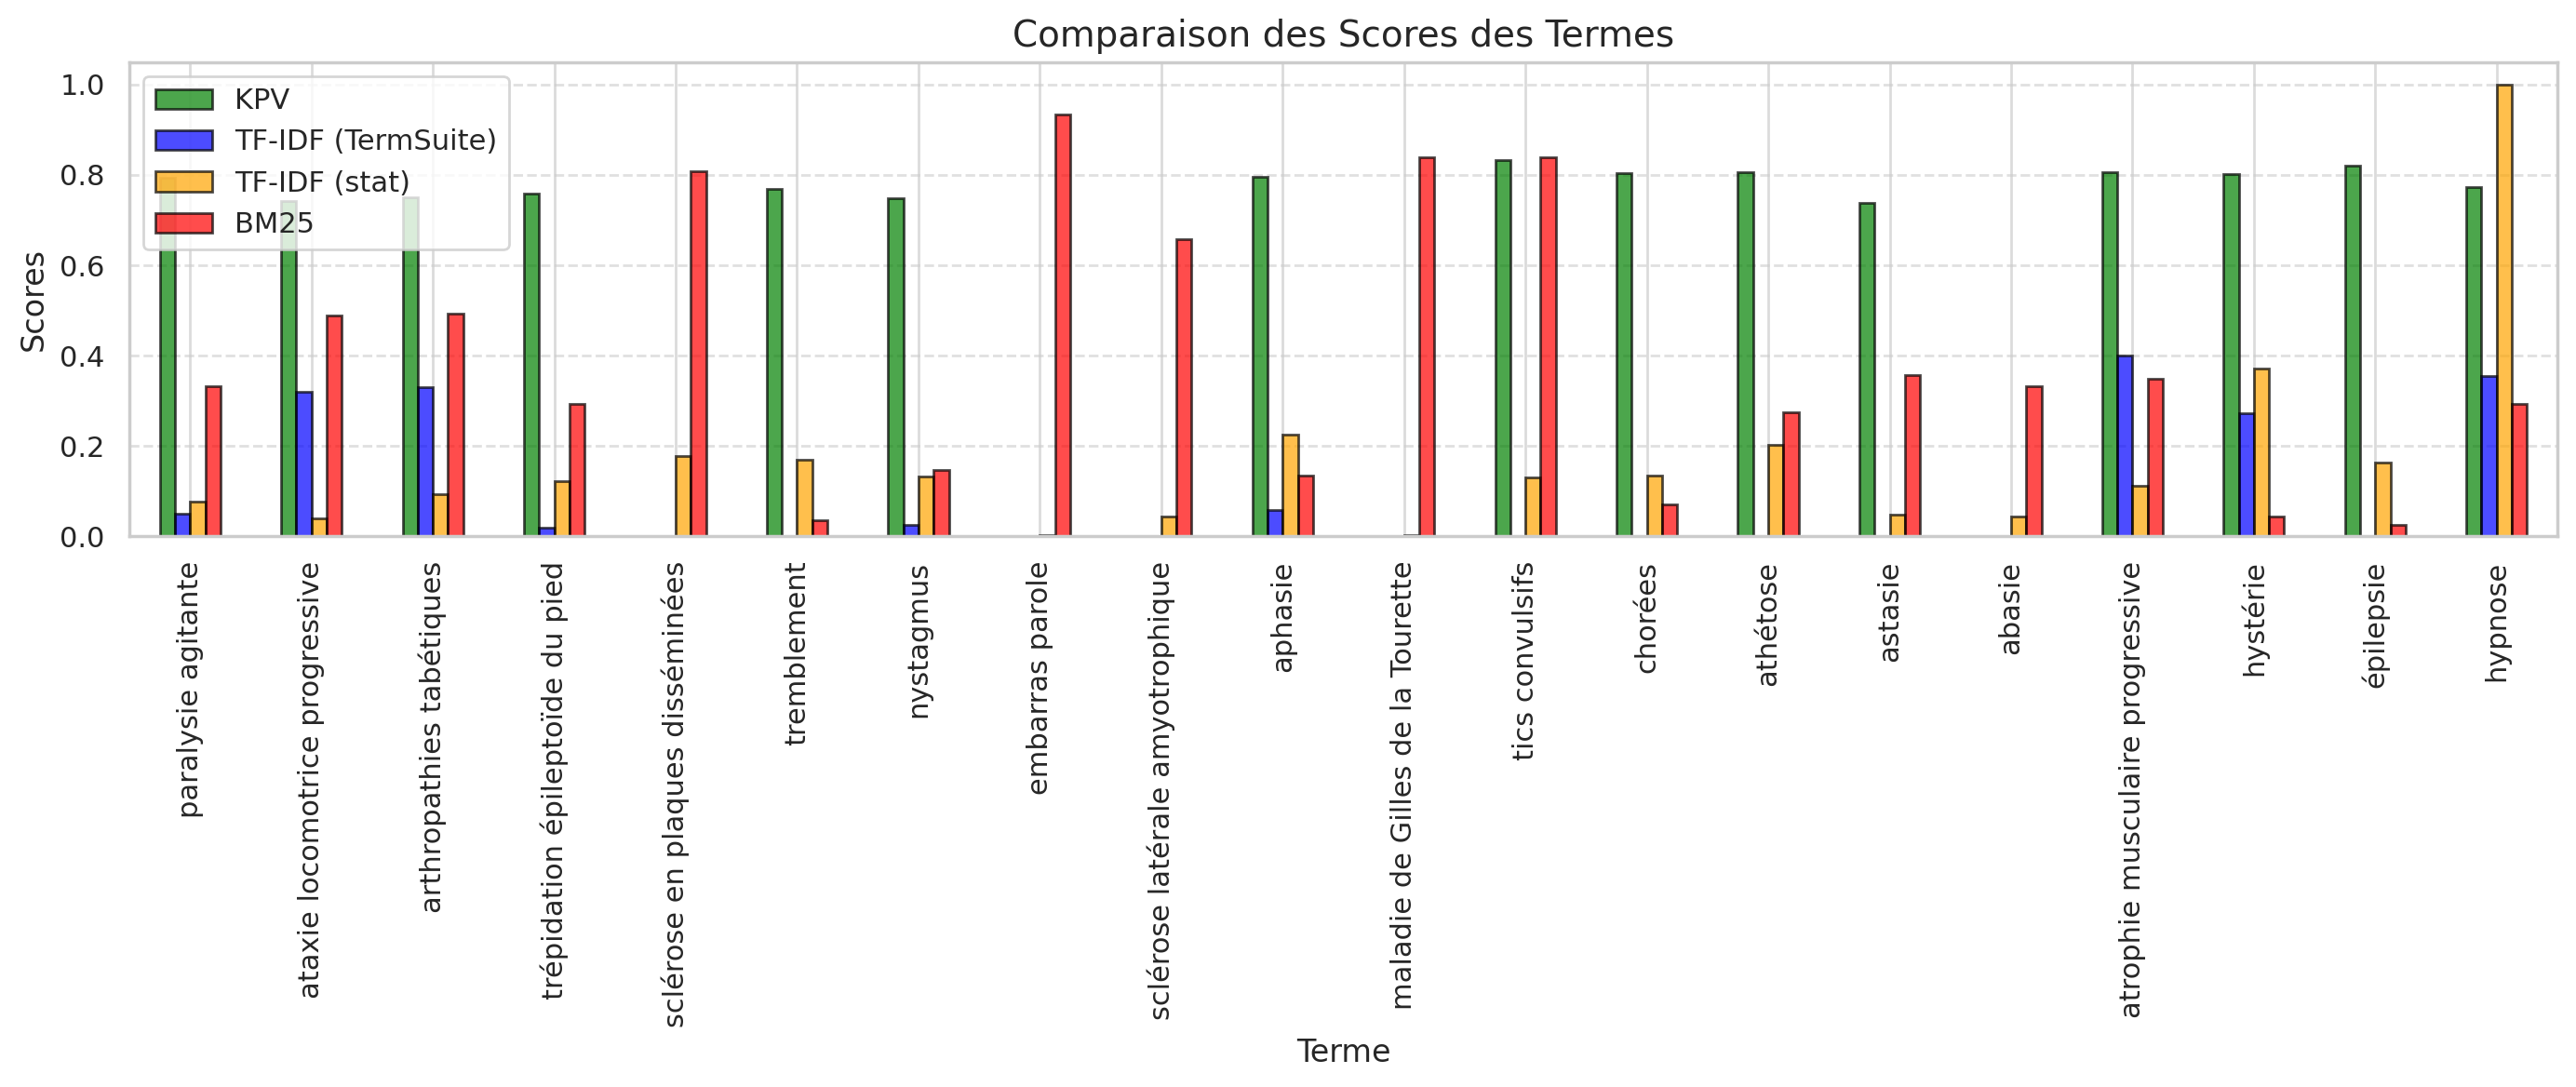
\includegraphics[width=\linewidth]{pic/termes_viz.png}
%	\caption{Visualisation des scores de pertinences pour chaque terme de référence}
%	\label{fig:ling_out_TAL}
%\end{figure}
%\end{frame}

%\begin{frame}{\textit{PatternRank}}
%	Les termes les plus pertinents dans \og{}Autres\fg{} :
%\begin{table}[h]
%	\centering
%	\begin{tabular}{|l|l|c|}
%		\hline
%		\textbf{Terme} & \textbf{Synonyme} & \textbf{Score} \\
%		\hline
%		\texttt{tics convulsifs} & \bolder{syndrome de Tourette} & \textsc{0.8331} \\
%		\texttt{état parkinsonien} & \bolder{maladie de Parkinson} & 0.7936 \\
%%		\texttt{paralytiques agitants} & \bolder{maladie de Parkinson} & 0.7851 \\
%		\hline
%	\end{tabular}
%\end{table}
%\end{frame}





%\begin{frame}{Chronologie d'une locution : indice de croissance de l'impact ?}
%\begin{figure}[h] % Use [H] to force the figure to stay in place
%	\begin{itemize}
%		\item évolution de la fréquence des termes au sein des deux corpus\footnote{\url{https://obtic.huma-num.fr/obvie/charcot/?view=corpus}}
%		\item convergence entre des termes : fin \textsc{XIX}\ieme{}, début \textsc{XX}\ieme{} s.
%%		\begin{itemize}
%%				\item \textit{ppm} : nombre d’occurrences par million de mots 
%%		\end{itemize}
%	\end{itemize}
%	\centering
%	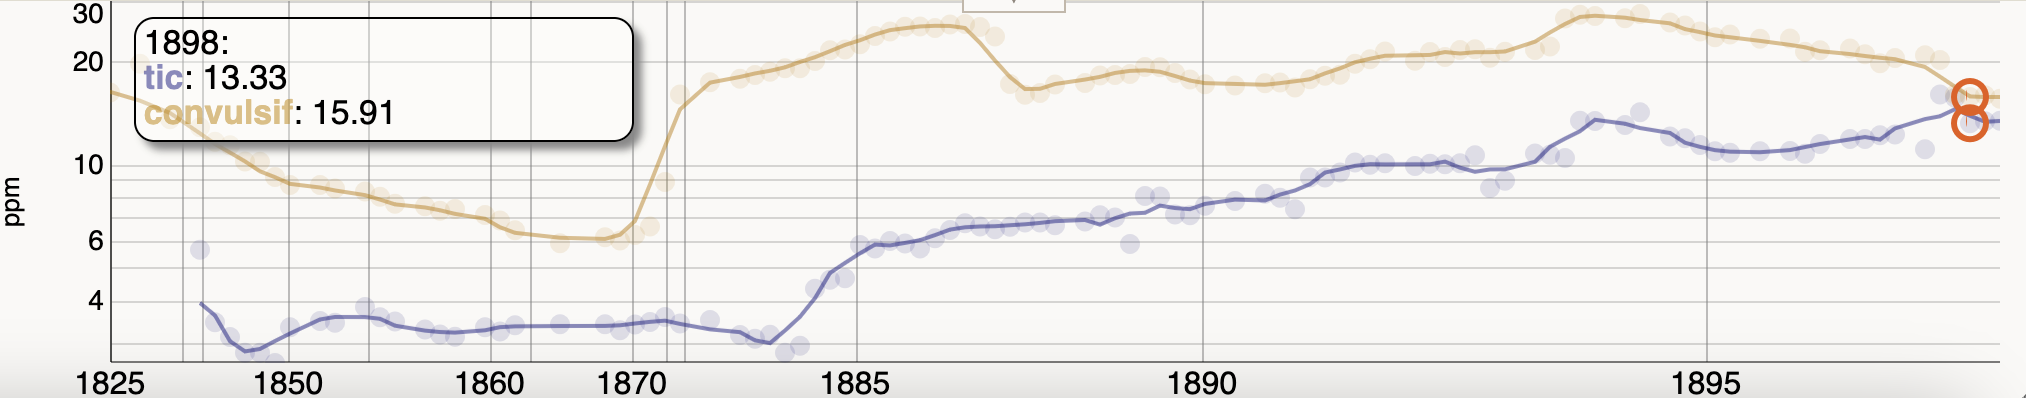
\includegraphics[width=\linewidth]{pic/tics_convulsifs.png}
%	\caption{Chronologie de la fréquence du terme \textit{tic convulsif}.}
%	\label{fig:ling_out_TAL}
%\end{figure}
%
%\begin{figure}[h]
%	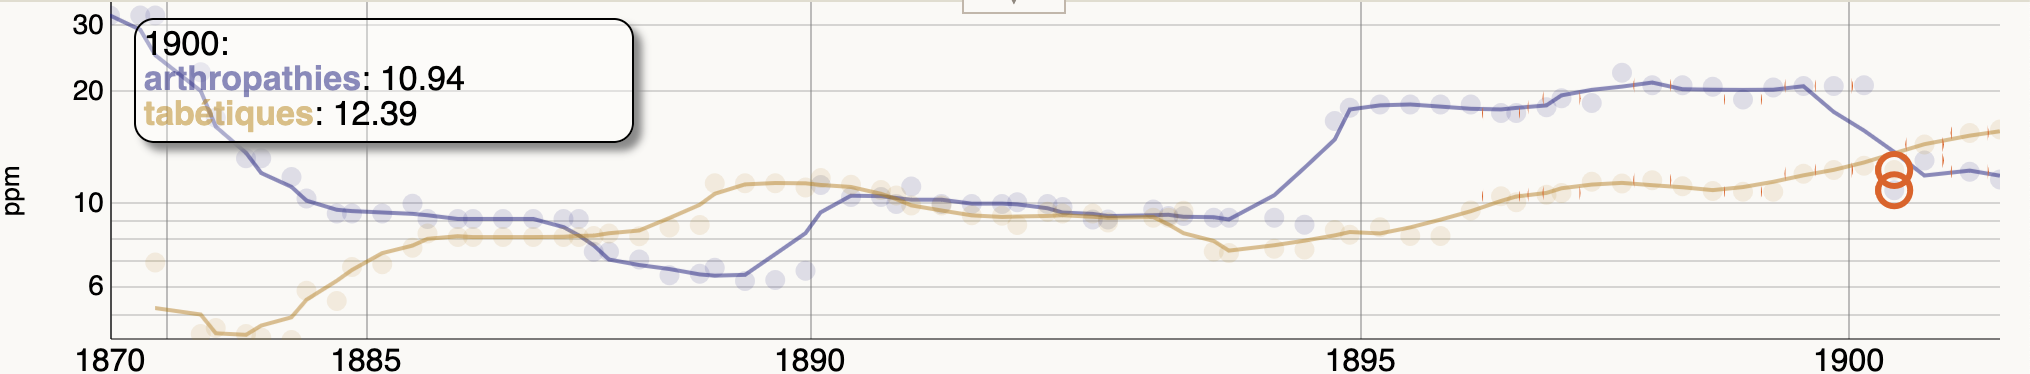
\includegraphics[width=\linewidth]{pic/arthropathies_tabetiques.png}
%\caption{Chronologie de la fréquence du terme \textit{arthropathies tabétiques}.}
%\label{fig:ling_out_TAL}
%\end{figure}
%\end{frame}


\section[Conclusion]{Conclusion}
\begin{frame}{Conclusion}
	\begin{enumerate}

%			\textit{PatternRank} : la méthode la plus fiable par rapport aux autres méthodes ?
%		\begin{itemize}
%			\item capture la sémantique jusqu'aux pentagrammes
%			\begin{itemize}
%%				\item quadrigrammes : \textit{sclérose cérébrale tubéreuse hypertrophique} 
%				\item \textit{méningite syphilitique hémorragique fibrineuse aiguë}
%			\end{itemize}
%			\item produit des scores de pertinence plus élevés
%			\begin{itemize}
%				\item exception : scores BM25 (\textit{SLA}, \textit{embarras parole}) et TF-IDF (\textit{hypnose})
%			\end{itemize}
		%\end{itemize}
\item \textit{PatternRank} : la méthode la plus fiable ($\neq$ \textit{TermSuite})
\begin{itemize}
	\item capture la sémantique jusqu'aux pentagrammes
\end{itemize}
		\item 	les termes les plus impactants dans les corpus :
		\begin{itemize}
			\item Charcot : \textit{hystérie}, \textit{astasie-abasie}, \textit{embarras parole}
			\item Autres :  \textit{hypnose}*, \textit{syndrome de Tourette}, \textit{arthropathies tabétiques}
		\end{itemize}
				\item absence occasionnelle de cooccurrent Charcot expliquable :
		\begin{itemize}
			\item \textit{épilepsie} : terme créé par J. H. Jackson
			\item \textit{hypnose} : terme créé par J. Braid
			\item \textit{athétose} : termée créé par W. A. Hammond
			\item \textit{chorées} : définition moderne par T. Sydenham
			\item \textit{trépidation épileptoïde du pied} : Babinski ? Vulpian? Charcot ? 			
		\end{itemize}

\begin{alertblock}{\vspace*{-0.6mm}}
	\centering
	Les résultats sont alignés avec les faits historiques.
\end{alertblock}

		
%		\item Absence des scores pour les termes comme \textit{SEP} et SLA :
%		\begin{itemize}                                        
%			\item solution : chercher leurs symptomes ou leurs descriptions :
%			\begin{itemize}
%				\item  \textit{amyotrophie spinale progressive}, \textit{secousses nystagmiques}$\dots$
%			\end{itemize}
%		\end{itemize}
	\end{enumerate}
	

		
	\end{frame}
%
%\section[Approche supervisée]{Approche supervisée}
%\input{2_methodo}
%\input{supervise}
%\section[Approche non supervisée]{Approche non supervisée}
%\input{non_supervise}
%\section[Conclusion]{Conclusion et recherches futures}
%\input{conclusion}
%\section[État de l'art]{État de l'art}
%\input{sota}
%\section[\textit{PatternRank}]{\textit{PatternRank}}
%\input{patternrank}



% \appendix

\begin{frame}[allowframebreaks]{Références}
\printbibliography

\end{frame}

\end{document}